%
\section{The Fundamental Algorithms within LocalRegions}

As stated in the introduction, this section of this guide is
structured in question-answer form.  This is not meant to capture
every possible question asked of us on the {\nek} users list; however,
this set of (ever-growing) questions are meant to capture the ``big
ideas'' that developers want to know about how LocalRegions work and
how they can be used.

In this section, we will through question and answer format try to
cover the following basic algorithmic concepts that are found within
the LocalRegions part of the library:

\subsection{Mapping trace data from an element face}

When handling discontinuous Galkerin (DG) expansions and techniques
such as Gradient Jump Penalisation we need to be able to take data
from the trace of the element (i.e. edges in 2D elements and faces in
3D element) to a unique trace which is shaped between two
elements. This is necessary for example to perform a Riemann problem
to link two elements in DG field. Such an action might require
interpolation from one distribution of quadrature points to another
however the shared trace space may not be aligned trivially with the
element trace.

In two-dimensions we only have edges which are either aligned so that
the local coordinate system runs in the same direction, noted by the
enum \verb+StdRegions::eForwards+ in the code, or in reverse
direction, noted by the enum \verb+StdRegions::eBackwards+ in the
code.

In three-dimensions the mappings get more complicated particularly for
quadrilateral faces. For triangular faces, our use of the collapsed
coordinate system means that triangular faces can only align in a
forwards or backwards sense because the singular vertices must align
and so this is managed in the mesh generation stage. For a triangular
faces we use the enum \verb+StdRegions::eDir1FwdDir1_Dir2FwdDir2+ to
denote a forwards aligned face and the enum
\verb+StdRegions::eDir1BwdDir1_Dir2FwdDir2+ to denote a face where
the bottom $x$-coordinate runs in the reverse of backwards direction
on the element trace compared to the shared trace.

At this point the meaning of the face enums needs a bit more
explanation. For any two-dimensional trace we have two coordinates
which are denoted by ``Dir1'' (Direction 1, i.e. $x$-direction) and
``Dir 2'' (Direction 2, i.e. $y$-direction). So the num
\verb+StdRegions::eDir1FwdDir1_Dir2FwdDir2+ denotes that direction 1
of the original triangle (or quadrilateral) is aligned to direction 1
of the shared/mapped triangle (or quadrilateral) and the two direction
are aligned (i.e. Forwards). It also denotes that direction 2 of the
original triangle (or quadrilateral) is aligned to direction 2 of the
shared/mapped triangle (or quadrilateral). The enum
\verb+StdRegions::eDir1BwdDir1_Dir2FwdDir2+ is similarly interpreted
but Direction 1 of the original face is now aligned to be in the
reverse direction to Direction 1 of the shared/mapped face.

For quadrilateral faces there are eight possible permutatiions that
one quadrilateral can be oriented to another quadrilateral and these include
\begin{itemize}
\item \verb+StdRegions::eDir1FwdDir1_Dir2FwdDir2+
\item \verb+StdRegions::eDir1FwdDir1_Dir2BwdDir2+
\item \verb+StdRegions::eDir1BwdDir1_Dir2FwdDir2+
\item \verb+StdRegions::eDir1BwdDir1_Dir2BwdDir2+
\item \verb+StdRegions::eDir1FwdDir2_Dir2FwdDir1+
\item \verb+StdRegions::eDir1FwdDir2_Dir2BwdDir1+
\item \verb+StdRegions::eDir1BwdDir2_Dir2FwdDir1+
\item \verb+StdRegions::eDir1BwdDir2_Dir2BwdDir1+
\end{itemize}

When coding we typically want to match the coefficients or physical
quadrature points from one face to another and so there are methods to
produce the mapping arrays to achieve this. For quadrature points we
have \verb+Expansion3D::ReOrientTracePhysMaps()+. In most cases there
is a symmetry as to whether you map from the element trace to the
shared trace or vice versa but for the two cases
\verb+StdRegions::eDir1FwdDir2_Dir2BwdDir1+
\verb+StdRegions::eDir1BwdDir2_Dir2FwdDir1+ where the faces are
transposed and one direction is reversed care must be taken since the
mappings are not symmetric. The method
\verb+Expansion3D::ReOrientTracePhysMaps()+ is defined by default to
provide a mapping which takes the local trace to the global trace such
that {\em sharedtrace[i] = localtrace[map[i]]}. However it is
possible to provide a false boolean to the argument \verb+Forwards+
and it will return the mapping from the shared trace to the local
trace so that {\em localtrace[i] = sharedtrace[map[i]]}. 

\begin{figure}[htb]
\centering
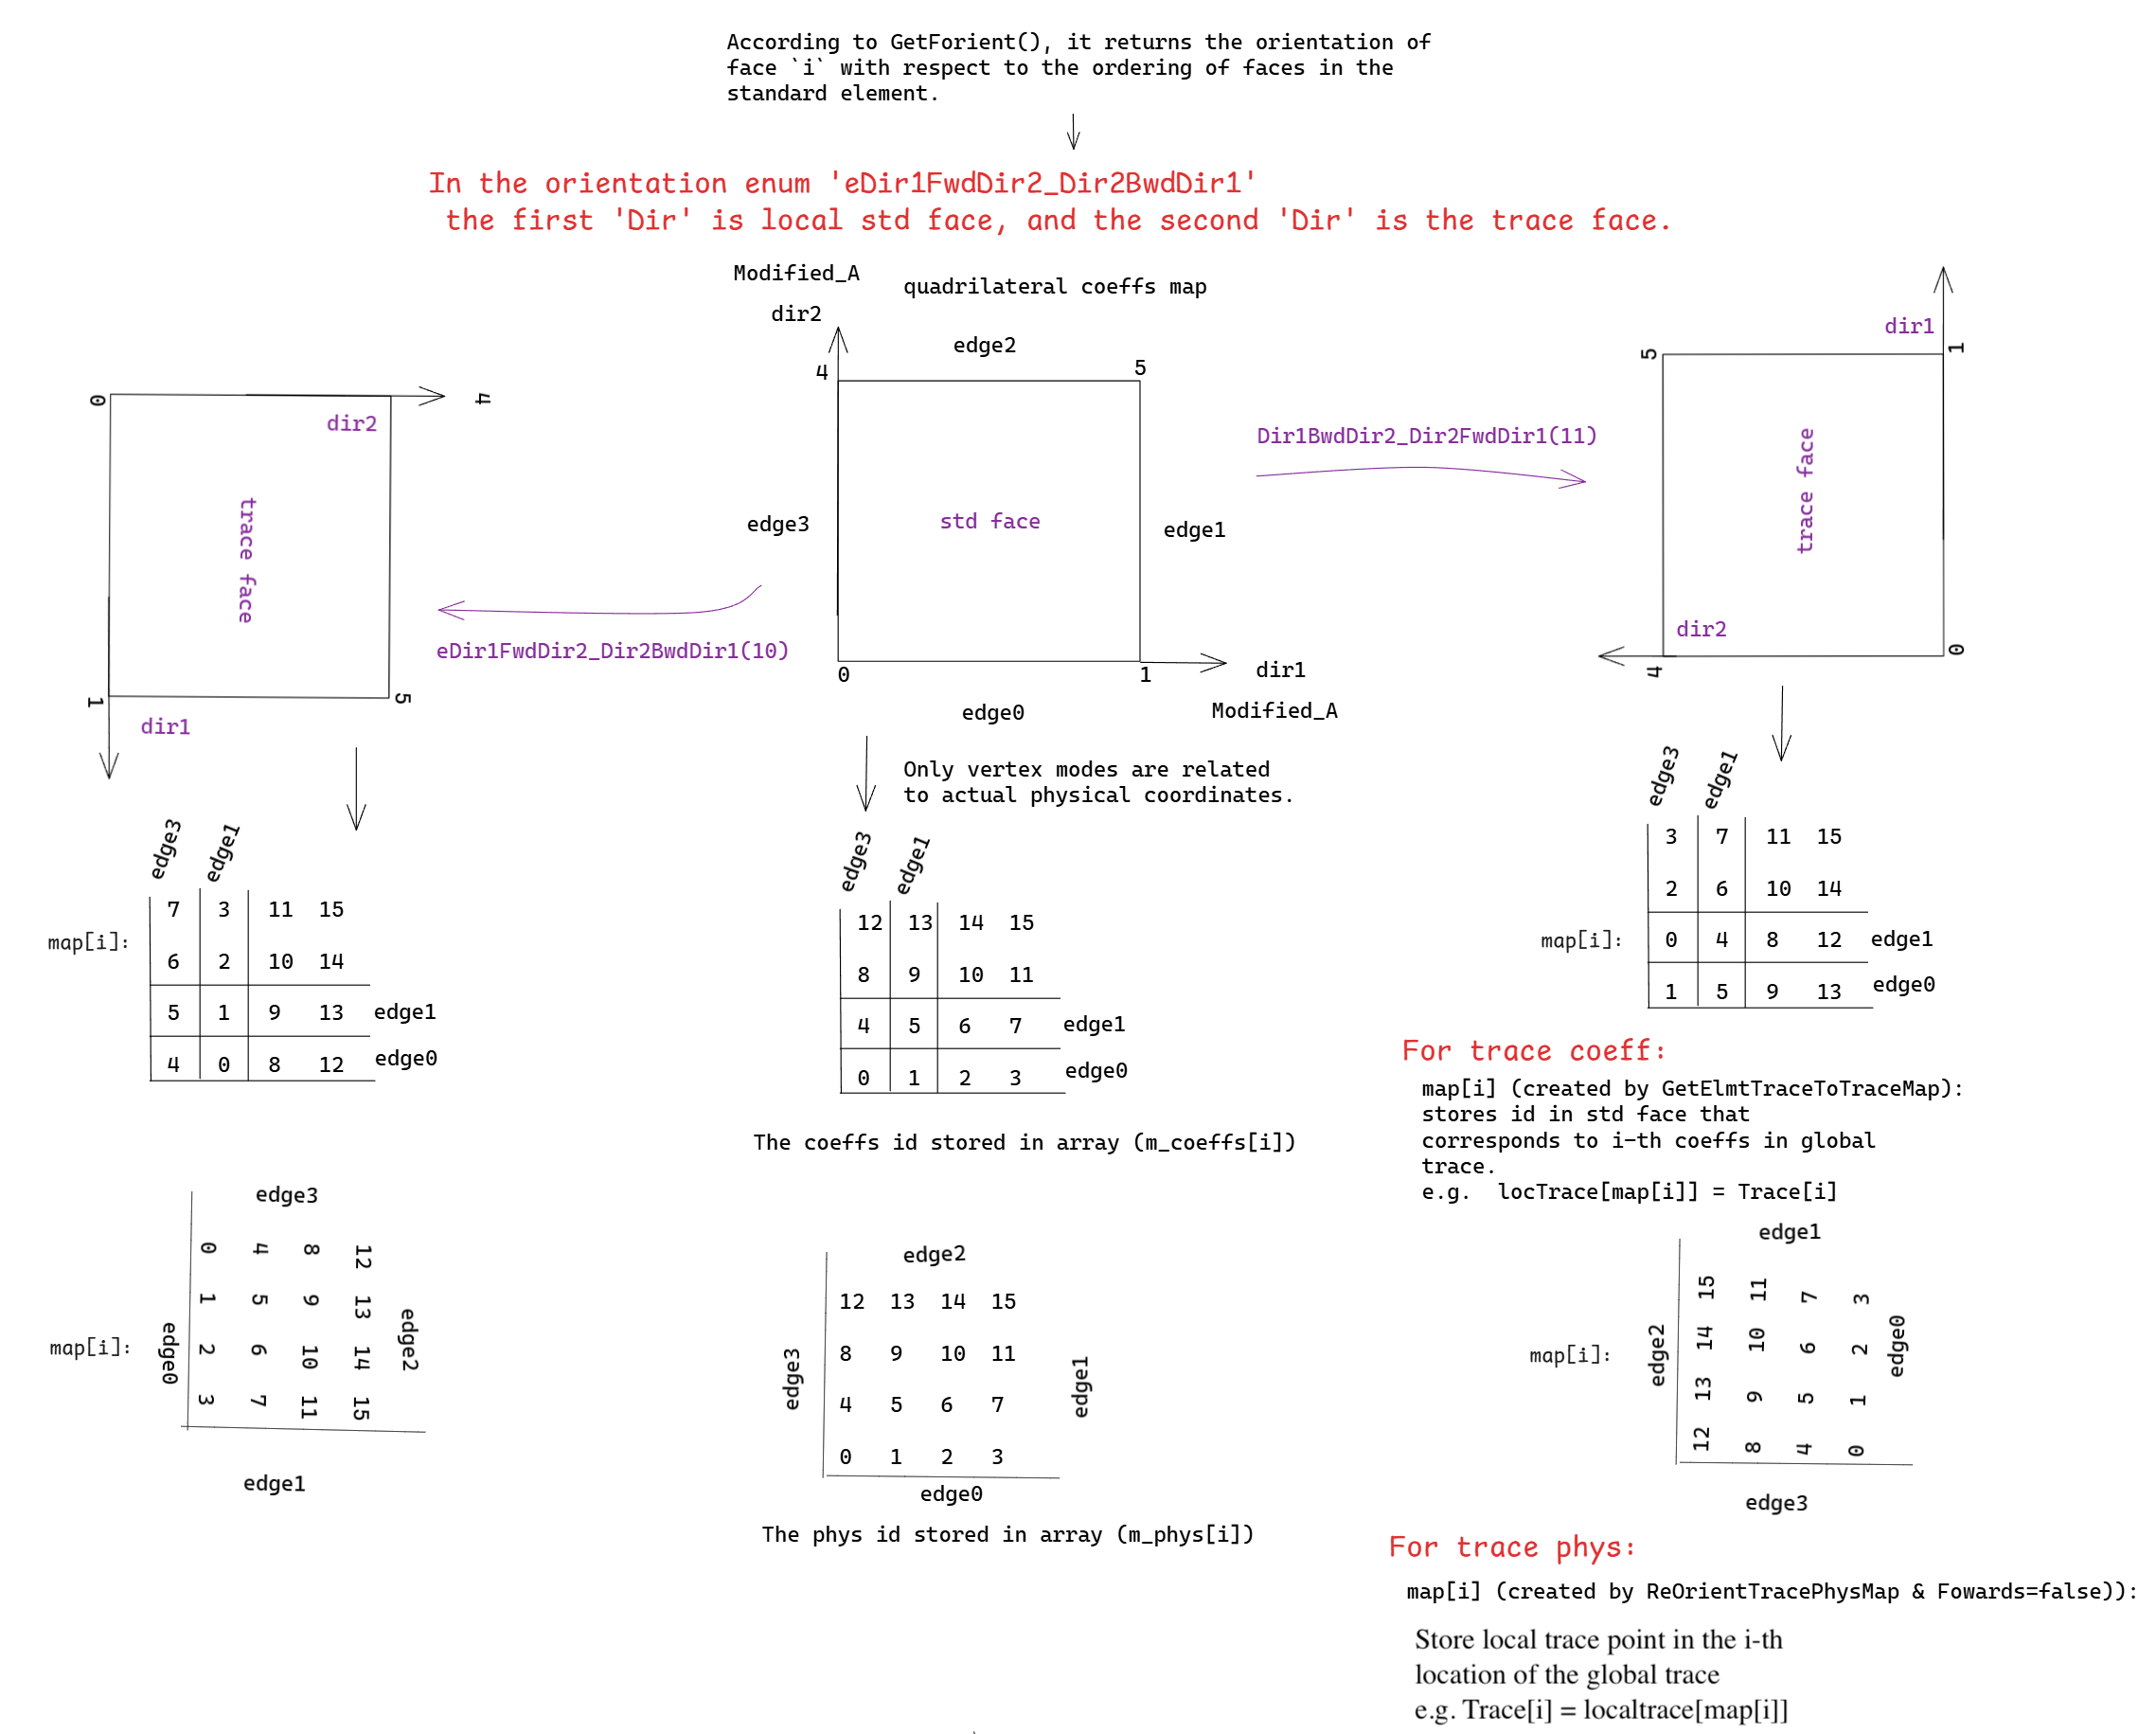
\includegraphics[width=5in]{img/TraceMap.png}
\caption{Example of trace mappings for complex transposed cases {\em eDir1FwdDir2\_Dir2BwdDir1} and {\em eDir1BwdDir2\_Dir2FwdDir1}.  }
\label{LocalRegions::TraceMap}
\end{figure}

Figure \ref{LocalRegions::TraceMap} provides an example of this more
complex mapping case for the reordering of the face coefficients and
also highlights the changes in the face orientation.

\subsection{Questions and Answers}
With the big ideas in place, let us now start into our questions.

\paragraph{Question:}
